\documentclass[11pt,a4paper]{amsart}
\usepackage[utf8]{inputenc}
\usepackage[T1]{fontenc}
\usepackage{amsmath,amssymb,amsthm}
\usepackage{graphicx}
\usepackage{booktabs}
\usepackage{longtable}
\usepackage{url}
\usepackage[margin=2.6cm]{geometry}
\usepackage[colorlinks=true,linkcolor=blue,citecolor=blue,urlcolor=blue]{hyperref}

\newtheorem{theorem}{Theorem}[section]
\newtheorem{lemma}[theorem]{Lemma}
\newtheorem{proposition}[theorem]{Proposition}
\newtheorem{corollary}[theorem]{Corollary}
\newtheorem{observation}[theorem]{Observation}
\theoremstyle{remark}
\newtheorem{remark}[theorem]{Remark}

\newcommand{\Q}{\mathbb{Q}}
\newcommand{\R}{\mathbb{R}}
\newcommand{\C}{\mathbb{C}}
\newcommand{\F}{\mathbb{F}}
\newcommand{\Euc}{\mathrm{E}(2)}

\title[New results around the Hadwiger--Nelson problem]{New results around the Hadwiger--Nelson problem:\\ probabilistic bounds, two forbidden distances,\\ map-type colourings and the unit sphere}
\author{Chrysovalantis Tsirindanis}
\address{School of Electrical and Computer Engineering, National Technical University of Athens, Greece}
\date{\today}

\begin{document}

\begin{abstract}
This document collects in one place the new results of the author on the chromatic number of the plane and three of its variants. They fall into three parts.

\emph{Part I (the probabilistic method beyond four colours).} For $d=(\sqrt2+\sqrt6)/2$ we prove $7\le\chi(\{1,d\})\le12$; the lower bound gives the first complete proof of a bound outlined in Polymath16, via an averaging argument and a $262$-point certificate checked by a machine-verified resolution proof. We give a vertex-critical $6$-chromatic $\{1,d\}$-graph with $30$ vertices (previous record $117$), and show by a $2$-adic computation that finite $\{1,d\}$-graphs in $\Q(i,\sqrt3,\sqrt m)$ are $4$-colourable whenever $m\equiv1,2,3,6\pmod8$, which covers $\Q(i,\sqrt3)$ itself. For proper $5$-colourings of the plane we obtain the first monochromatic-pair bounds, $2p^{(5)}_{\sqrt3}+p^{(5)}_2\ge\frac23$, $p^{(5)}_{\sqrt3}\ge\frac1{12}$, $p^{(5)}_{\sqrt7}\le\frac49$, and we improve two entries of the Polymath16 table for $4$-colourings: $p^{(4)}_{\sqrt7}\le\frac13$ and $p^{(4)}_2\ge0.2886964$.

\emph{Part II (map-type colourings).} We answer Question~1 of Sokolov and Voronov: the radius their argument needs is exactly $\rho+2$, the optimal convex region is a disc, and $\rho\le1/\sqrt3$, so the area drops from $9\pi$ to $\pi(2+1/\sqrt3)^2$. We also prove, by a parity argument, a step their proof asserts without proof, and isolate one case it does not cover.

\emph{Part III (the unit sphere).} The largest set of points on $S^2(1)$ whose chord-$1$ graph has independence number at most $2$ has exactly $7$ points, i.e.\ $\alpha(3,\tfrac12)=7$, and the extremal configuration is unique.
\end{abstract}

\maketitle
\tableofcontents

\section{Introduction and summary}

The Hadwiger--Nelson problem asks for $\chi(\R^2)$, the least number of colours for the plane with no two points at distance $1$ of the same colour. Since de Grey's construction~\cite{dG18} the bounds are $5\le\chi(\R^2)\le7$. This document does not move these bounds. It collects new results on four questions around them, obtained by the author in 2026. Each part is self-contained; the parts share only the introduction, the bibliography and the list of open problems in Section~\ref{sec:open}.

\begin{center}
\small
\begin{tabular}{p{6.2cm}p{2.6cm}p{4.6cm}}
\toprule
Result & Where & Status\\
\midrule
$\chi(\{1,(\sqrt2+\sqrt6)/2\})\ge7$ & Thm.~\ref{thm:seven} & proof + verified certificate; first complete proof of a Polymath16 outline\\
$\chi(\{1,(\sqrt2+\sqrt6)/2\})\le12$ & Prop.~\ref{prop:upper} & elementary, not new in substance\\
$6$-chromatic $\{1,d\}$-graph, $30$ vertices & Thm.~\ref{thm:g30} & new record (previous $117$)\\
Finite $\{1,d\}$-graphs in $\Q(i,\sqrt3,\sqrt m)$ are $4$-colourable for $m\equiv1,2,3,6\ (8)$ & Prop.~\ref{prop:mod8} & proof\\
Limits of the ``exactly $\tfrac12$'' method & Prop.~\ref{prop:limits} & proof\\
$2p^{(5)}_{\sqrt3}+p^{(5)}_2\ge\frac23$, $p^{(5)}_{\sqrt3}\ge\frac1{12}$, $p^{(5)}_{\sqrt7}\le\frac49$, $\sup_{0<\delta<2}p^{(5)}_\delta\ge\frac14$ & Section~\ref{sec:five} & proof (exact enumeration)\\
$p^{(4)}_{\sqrt7}\le\frac13$ (was $\frac{37}{100}$), $p^{(4)}_2\ge0.2886964$ (was $\frac14$) & Thms.~\ref{thm:p7four}, \ref{thm:p2four} & proof; LP certificate\\
Which Polymath16 lemmas survive at $k=5$ & Section~\ref{sec:survive} & classification\\
Obstruction radius $\rho+2$, optimal region a disc, $\rho\le1/\sqrt3$ & Section~\ref{sec:radius} & proof\\
An eleventh trichromatic point, odd count & Thms.~\ref{thm:eleventh}, \ref{thm:odd} & proof of a step asserted in~\cite{SV26,Vo24}\\
$\alpha(3,\frac12)=7$, unique extremal set & Section~\ref{sec:sphere} & proof (Ramsey, Gr\"obner basis, exhaustion)\\
\bottomrule
\end{tabular}
\end{center}

\medskip
\noindent\textbf{On attribution.} Most tools used here belong to others: the probabilistic formulation (Tao, Polymath16), the linear-programming pipeline (Mixon and Alexeev), the $8$-point gadget and the observation on $p_\delta=\tfrac12$ (Parts and de Grey, Polymath16), the spindle construction on the sphere (Bachoc, Bekker, Moustrou and de Oliveira Filho), and the framework for map-type colourings (Sokolov and Voronov). The precise attributions are given where each is used.

\part{The probabilistic method beyond four colours}

\section{The averaging framework}\label{sec:avg}

Let $D\subset(0,\infty)$ be a set of forbidden distances and $c\colon\R^2\to\{1,\dots,k\}$ a colouring with no monochromatic pair at a distance in $D$. Let $\Euc$ be the isometry group of the plane, viewed as a discrete group. It is solvable ($\R^2\rtimes O(2)$ with $O(2)=SO(2)\rtimes C_2$), hence amenable~\cite{Ru02}. So there is a left-invariant mean on $\ell^\infty(\Euc)$; composing it with $g\mapsto g^{-1}$ gives a mean $\mu$ (a positive linear functional with $\mu(1)=1$) with $\mu(f(\cdot\,h))=\mu(f)$. Equivalently, $\mu$ is a finitely additive probability measure on all subsets of $\Euc$. This is the setting of Polymath16 (Tao) and of \'Agoston~\cite[\S4.1]{Ag21}, who use a left-invariant measure on $S_k\times\Euc$ and the random colouring $\sigma\circ c\circ T^{-1}$. No measurability of $c$ is assumed. For points $A,B$ put
\[
f_{A,B}(g)=\mathbf 1\bigl[c(gA)=c(gB)\bigr],\qquad g\in\Euc .
\]
Then $f_{hA,hB}(g)=f_{A,B}(gh)$, so $\mu(f_{A,B})$ depends only on $|AB|$; write $p_{|AB|}$, or $p^{(k)}_{|AB|}$ when the number of colours matters. Only linearity, positivity and $\mu(1)=1$ are used: if $\sum_j f_j\ge m$ pointwise then $\sum_j\mu(f_j)\ge m$.

\begin{lemma}[{\cite[Prop.~4.2.1]{Ag21}; Lemma~2 of the Polymath16 wiki}]\label{lem:half}
If $1\in D$, then for every $k$ and every $\delta\ge\tfrac12$, $p_\delta\le\tfrac12$.
\end{lemma}

\begin{proof}
Take $P,Q,R$ with $|PQ|=|PR|=\delta$ and $|QR|=1$. Since $c(gQ)\ne c(gR)$ for every $g$, $f_{P,Q}+f_{P,R}\le1$, so $2p_\delta\le1$.
\end{proof}

\begin{remark}[on the strict inequality]\label{rem:strict}
The strict inequality $p_\delta<\tfrac12$ for $\delta>\tfrac12$ was sketched for every number of colours by P\'alv\"olgyi in the twelfth Polymath16 thread~\cite{PM12}; \'Agoston proved it for $4$ colours and remarked that a chain of isosceles triangles should extend it~\cite[Prop.~4.2.6, Rem.~4.2.7]{Ag21}. A written proof for more than four colours does not seem to be available. Nothing in this document uses it.
\end{remark}

\section{Monochromatic-pair bounds for five colours}\label{sec:five}

Here $D=\{1\}$. The Polymath16 project assembled a table of bounds on $p^{(4)}_\delta$ for a hypothetical proper $4$-colouring. As de Grey observed in 2019, for more colours the only facts on record were $p_1=0$ and the bounds of Lemma~\ref{lem:half} and Remark~\ref{rem:strict}. We run the existing machinery at $k=5$.

\subsection{Which lemmas survive}\label{sec:survive}

Ask of each lemma of the Polymath16 wiki what role the number of colours plays in its \emph{proof}.

\begin{center}
\small
\begin{tabular}{p{3cm}p{6cm}p{4.4cm}}
\toprule
class & mechanism & at $k=5$\\
\midrule
$k$-free & counts no colours, only incompatibility & transfers verbatim\\
$k$ in the constant & argument intact, one numerical input changes & recomputed below\\
$k$ in the structure & pigeonhole over $k+1$ points, or the four $4$-colourings of a gadget & collapses\\
\bottomrule
\end{tabular}
\end{center}

The first class contains L2 (Lemma~\ref{lem:half}), L12, L17 ($p_a+p_b\le1+p_c$), L34, L38, and L30/C31/L32; the second, Corollary~16 and its descendants; the third, L15, C16, L19, L22, L23--L27, P35 and P36. Lemma~38 is the one used below: for a unit equilateral triangle $ABC$ and any point $D$, at most one of $AD,BD,CD$ is monochromatic, so $p_{|AD|}+p_{|BD|}+p_{|CD|}\le1$; no colour is counted. Every improvement of $p_\delta\le\tfrac12$ on record ($\tfrac12-\tfrac1{62}$, $0.48$, $\tfrac{323}{675}$) is in the third class and is lost at $k=5$.

A lemma can look $k$-free and not be. Chroman's inequality $1\le p_v+p_w+p_x+p_y+p_z\le2$ for the diagonals of an equilateral pentagon never mentions four, but its lower half is a pigeonhole over five points and four colours. \emph{The criterion is whether $k$ appears in the proof, not in the statement.} Its $k=5$ analogue needs six points:

\begin{lemma}[hexagon lemma]\label{lem:hexagon}
Let $ABCDEF$ be a closed hexagon with unit sides and $d_1,\dots,d_9$ the lengths of its diagonals. Then $\sum_{i=1}^9p^{(5)}_{d_i}\ge1$.
\end{lemma}

\begin{proof}
Six points, five colours: some pair is monochromatic; sides are unit, so the pair is a diagonal. Take expectations.
\end{proof}

For the regular hexagon this reads $2p_{\sqrt3}+p_2\ge\tfrac13$, weaker than Theorem~\ref{thm:wheel}. Among $2\times10^5$ random closed unit hexagons, $72{,}563$ had nine distinct diagonal lengths, six had eight and none fewer; a useful instance needs a hexagon whose diagonals take two or three values, which we leave open.

\subsection{The table at $k=5$}

Let $H$ be the wheel $W_6$: a centre joined to a rim $C_6$ of unit edges ($7$ vertices, $12$ unit edges). Its non-unit pairs are six rim pairs at distance $\sqrt3$ and three antipodal pairs at distance $2$. For a colouring let $a$ and $b$ be the numbers of monochromatic $\sqrt3$- and $2$-pairs; then $\mathbb E[a/6]=p_{\sqrt3}$ and $\mathbb E[b/3]=p_2$, and every inequality $\alpha(a/6)+\beta(b/3)\ge\gamma$ valid for all proper colourings of $H$ gives $\alpha p_{\sqrt3}+\beta p_2\ge\gamma$.

\begin{theorem}\label{thm:wheel}
$2p^{(5)}_{\sqrt3}+p^{(5)}_2\ge\tfrac23$, and this is the only non-redundant inequality $H$ gives in these coordinates.
\end{theorem}

\begin{proof}
The proper $5$-colourings of $H$ give eight points $(a/6,b/3)$. The Pareto minima are $(0,\tfrac23)$, $(\tfrac16,\tfrac13)$, $(\tfrac13,0)$; they are collinear, so the lower-left hull has the single facet $x/(1/3)+y/(2/3)=1$.
\end{proof}

At $k=4$ the same computation gives four points, minima $(0,1),(\tfrac13,\tfrac13),(\tfrac23,0)$ and two facets $2p_{\sqrt3}+p_2\ge1$, $p_{\sqrt3}+p_2\ge\tfrac23$ (Lemma~15 of the wiki; de Grey's four states). Passing from four colours to five costs a constant and a facet.

\begin{theorem}\label{thm:p3five}
$p^{(5)}_{\sqrt3}\ge\tfrac1{12}$.
\end{theorem}
\begin{proof}
$p_2\le\tfrac12$ by Lemma~\ref{lem:half}; substitute into Theorem~\ref{thm:wheel}.
\end{proof}

\begin{theorem}\label{thm:p7five}
$p^{(5)}_{\sqrt7}\le\tfrac49$.
\end{theorem}
\begin{proof}
Lemma~38 applied to the configurations with $(|AD|^2,|BD|^2,|CD|^2)=(3,4,7)$ (e.g.\ $A=(0,0)$, $B=(1,0)$, $C=(\tfrac12,\tfrac{\sqrt3}2)$, $D=(0,-\sqrt3)$) and $(3,7,7)$ gives $p_{\sqrt3}+p_2+p_{\sqrt7}\le1$ and $p_{\sqrt3}+2p_{\sqrt7}\le1$. Adding, $2p_{\sqrt3}+p_2+3p_{\sqrt7}\le2$; with Theorem~\ref{thm:wheel}, $3p_{\sqrt7}\le\tfrac43$.
\end{proof}

\begin{theorem}[correction at $k=4$]\label{thm:p7four}
$p^{(4)}_{\sqrt7}\le\tfrac13$, improving $\tfrac{37}{100}$ in the Polymath16 table.
\end{theorem}
\begin{proof}
From the $(3,4,7)$ instance, $p_{\sqrt7}\le1-(p_{\sqrt3}+p_2)$, and $p^{(4)}_{\sqrt3}+p^{(4)}_2\ge\tfrac23$.
\end{proof}

\begin{proposition}\label{prop:sup}
$\sup_{0<\delta<2}p^{(5)}_\delta\ge\tfrac14$.
\end{proposition}
\begin{proof}
The points $e^{2\pi ij/n}$ are at distance $1$ from the origin, so they use at most four colours. With class sizes $n_1,\dots,n_4$ there are $\sum n_i(n_i-1)/2\ge n^2/8+O(n)$ monochromatic pairs among $\binom n2$; take expectations and let $n\to\infty$.
\end{proof}

All constants above were recomputed in exact rational arithmetic (enumeration of the colourings of $W_6$, exact hull facets).

\subsection{An LP certificate at $k=4$}

\begin{theorem}[correction at $k=4$]\label{thm:p2four}
$p^{(4)}_2\ge\tfrac{2838001}{9830400}=0.2886964\ldots$, improving $\tfrac14$.
\end{theorem}

\noindent\emph{The graph.} With $\omega_1=e^{i\pi/3}$, $\omega_3=(5+i\sqrt{11})/6$, $\mathrm{hex}=\{0,1,\omega_1,1+\omega_1,\bar\omega_1,1+\bar\omega_1,2\}$ and $v=1+\omega_1$, let
\[
G_{19}=\mathrm{hex}\cup\omega_3\cdot\mathrm{hex}\cup\{v+\omega_3(p-v):p\in\mathrm{hex}\}.
\]
It has $19$ vertices and $45$ unit edges; its $126$ non-unit pairs fall into $28$ distance classes; it has $3098$ monochromatic profiles of proper $4$-colourings. (Adjoining $2+\omega_1$ and $3$ gives Parshall's $21$-vertex graph; deleting four vertices gives the $17$-vertex graph $G_{17}$ of Mixon and Alexeev, which yields $0.2775182\ldots$ by the same method.)

\noindent\emph{The linear program} (Mixon--Alexeev). For the set $P$ of profiles, a random proper $4$-colouring of the plane induces a probability vector $w$ on $P$ with $\sum_r w_rr_e=p_{|e|}$ for every non-unit pair $e$. Minimising $p_2$ over such $w$, with the consistency constraint imposed on all $28$ classes, gives a valid lower bound. By duality it suffices to exhibit $y\in\Q^{126}$, $t\in\Q$ with (C1) $t+\sum_{e:\,r_e=1}y_e\le0$ for every profile $r$ and (C2) $-\sum_{e\in c}y_e\le[c=\text{class of }2]$ for every class $c$; then $p_2\ge t$. Such a certificate with $t=2838001/9830400$ is in the ancillary file \texttt{certificate19.json} and is checked in exact arithmetic by \texttt{check\_certificate19.py}, which rebuilds $G_{19}$ and its profiles independently of any LP solver. The LP optimum on $G_{19}$ is $0.2887084\ldots$. If $y$ is required to be constant on classes the dual optimum collapses to $0$: the bound comes from weighting pairs of the same length differently according to their position.

\subsection{A calibrated negative}

On $G_{17}$, restricted to the classes $\{\sqrt3,2\}$, the LP reproduces $p^{(4)}_2\ge\tfrac14$ exactly ($228$ profiles, the number Mixon reports). At $k=5$ the same two classes give $4418$ profiles and lower bound $0$ for both; adding the rational classes $\{\tfrac13,\tfrac53,\tfrac43\}$ gives $176{,}371$ profiles and still $0$. This is expected: at $k=4$ each colour class would need density $\tfrac14$, above the upper bound $\approx0.2415$ for measurable $1$-avoiding sets, while at $k=5$ it needs $\tfrac15$, below Croft's lower bound $0.22936$; there is no density pressure for a small graph to detect.

In the same direction, Tao's origin-forcing lemma (thread~5) needs a graph whose origin is non-bichromatic. Rebuilding the Polymath16 family (Minkowski powers of $\{\omega_1^a\omega_3^b:0\le a\le5,\ |b|\le1\}$) in exact arithmetic over $\Q(\sqrt3,\sqrt{11})$, the origin is forced at $k=4$ from the third power on ($865$ vertices, $4530$ unit edges; a vertex-critical $48$-vertex subgraph suffices), but at $k=5$ it is forced neither there nor at the fourth power ($3313$ vertices, $21{,}900$ edges).

\section{Two forbidden distances: \texorpdfstring{$7\le\chi(\{1,(\sqrt2+\sqrt6)/2\})\le12$}{7 <= chi <= 12}}\label{sec:two}

Here $D=\{1,d\}$ with $d=(\sqrt2+\sqrt6)/2$, so $d^2=2+\sqrt3$. A finite point set joined at distances $1$ and $d$ is a \emph{$\{1,d\}$-graph}. The bound $\chi(\{1,d\})\ge6$ is known for $d=2$ (Exoo--Ismailescu~\cite{EI19}), $d=(1+\sqrt5)/2$ (Huddleston; a $16$-vertex proof is due to Parts~\cite{Pa20}), and for $d=\sqrt3$ and $d=(\sqrt3+1)/\sqrt2=(\sqrt2+\sqrt6)/2$, first by P\'alv\"olgyi and \'Agoston with a probabilistic argument (see~\cite{Pa20}) and then with explicit graphs of $33$ and $117$ vertices by De Neve, Vanden Kerchove, Colle, Tavernier and Pickavet~\cite{DN25}.

For our $d$, the bound $\chi\ge7$ was argued in outline in the fifteenth Polymath16 thread~\cite{PM15}: Parts proposed the $8$-point gadget of Lemma~\ref{lem:gadget} (24 December 2019), and de Grey observed that if some $p_\delta=\tfrac12$ then every isosceles triangle with legs $\delta$ and base $1$ has a monochromatic leg (28 December 2019). The gadget appears there only as an image and the argument only in words. The shortest completion would use the strict inequality of Remark~\ref{rem:strict} for six colours, which is only sketched. We instead make de Grey's observation effective with a finite certificate.

\begin{theorem}\label{thm:seven}
$\chi(\{1,(\sqrt2+\sqrt6)/2\})\ge7$.
\end{theorem}

\subsection{The gadget}

\begin{lemma}[gadget]\label{lem:gadget}
Let $\zeta=e^{i\pi/6}$ and $X=\{0,\,1,\,i,\,1+\zeta,\,1+i,\,\zeta^5,\,\zeta^{10},\,\zeta^2+i\}\subset\mathbb C$. All $28$ pairs of $X$ except the four pairs
\[
(1,i),\quad(1+i,0),\quad(1+\zeta,\zeta^5),\quad(\zeta^{10},\zeta^2+i)
\]
are at distance $1$ or $d$. The first two of these pairs are at distance $\sqrt2$ and the last two at distance $1+\sqrt3$. Consequently, if $k=6$ then $2p_{\sqrt2}+2p_{1+\sqrt3}\ge2$.
\end{lemma}

\begin{proof}
The distances are checked by direct computation (we verified them in exact arithmetic). For each $g$, the map $x\mapsto c(gx)$ properly colours the graph on $X$ whose edges are the $24$ forbidden pairs. Its complement is a perfect matching, so each colour class has at most two points, and a class with two points is one of the four matched pairs. Eight points in at most six classes give at least two such classes. Hence the four indicators sum to at least $2$ pointwise, and we apply $\mu$.
\end{proof}

\begin{corollary}\label{cor:equal}
If $k=6$, then $p_{\sqrt2}=p_{1+\sqrt3}=\tfrac12$.
\end{corollary}

\begin{proof}
Combine Lemmas~\ref{lem:half} and~\ref{lem:gadget}.
\end{proof}

\subsection{Rigid triangles and the proof}

Call a triple $(P;Q,R)$ of points a \emph{rigid triangle} if $|PQ|=|PR|\in\{\sqrt2,\,1+\sqrt3\}$ and $|QR|\in\{1,d\}$.

\begin{lemma}\label{lem:finite}
Suppose $k=6$. Let $F$ be a finite point set and $\mathcal T$ a finite set of rigid triangles with vertices in $F$. Then there is a colouring $\phi\colon F\to\{1,\dots,6\}$ such that
\begin{enumerate}
\item $\phi(x)\ne\phi(y)$ whenever $|xy|\in\{1,d\}$, and
\item $\phi(P)=\phi(Q)$ or $\phi(P)=\phi(R)$ for every $(P;Q,R)\in\mathcal T$.
\end{enumerate}
\end{lemma}

\begin{proof}
Fix $t=(P;Q,R)\in\mathcal T$ and let $\delta=|PQ|$. Because $|QR|\in\{1,d\}$, $f_{P,Q}f_{P,R}=0$, so $N_t:=1-f_{P,Q}-f_{P,R}$ takes values in $\{0,1\}$. By Corollary~\ref{cor:equal}, $\mu(N_t)=1-2p_\delta=0$. If every $g$ had $N_t(g)=1$ for some $t$, then $\sum_t N_t\ge1$ pointwise and $0=\sum_t\mu(N_t)\ge1$, which is absurd. Pick $g$ with $N_t(g)=0$ for all $t$ and set $\phi(x)=c(gx)$.
\end{proof}

\begin{proposition}\label{prop:cert}
There is a set $F$ of $262$ points in $\Q(i,\sqrt3,\sqrt7)$ and a set $\mathcal T$ of $248$ rigid triangles with vertices in $F$ for which no colouring $\phi$ as in Lemma~\ref{lem:finite} exists.
\end{proposition}

The configuration and its verification are described in Section~\ref{sec:cert}.

\begin{proof}[Proof of Theorem~\ref{thm:seven}]
A proper $6$-colouring of the plane would, by Lemma~\ref{lem:finite}, give a colouring $\phi$ of the set $F$ of Proposition~\ref{prop:cert}, which does not exist. A colouring with fewer than $6$ colours is in particular a $6$-colouring.
\end{proof}

\begin{remark}
The $\{1,d\}$-graph on $F$ alone is $6$-colourable (an explicit colouring was found and checked). Thus neither ingredient suffices by itself: the averaging argument supplies the triangle constraints, and the finite set makes them contradictory.
\end{remark}

\subsection{The certificate}\label{sec:cert}

Let $\omega=(3+i\sqrt7)/4$, a unit complex number of argument $\arccos(3/4)$. For a rigid triangle with legs $\sqrt2$ and base $1$ the apex angle is exactly $\arg\omega$, so such triangles need $\sqrt7$. In fact the field $\Q(\zeta)=\Q(i,\sqrt3)$ contains no rigid triangle: the apex angle $\theta$ of a rigid triangle has $\cos\theta\in\{\tfrac34,\tfrac{2+\sqrt3}4,\tfrac{2-\sqrt3}4\}$, and $e^{i\theta}=(R-P)/(Q-P)$ would lie in $\Q(\zeta)$, forcing $\sin\theta\in\Q(\sqrt3)$; but $16\sin^2\theta\in\{7,\,9-4\sqrt3,\,9+4\sqrt3\}$, none of which is a square in $\Q(\sqrt3)$.

\medskip\noindent\textbf{Construction.} Let $U=\{\zeta^k\omega^a:0\le k<12,\ a\in\{-1,0,1\}\}$ ($36$ unit vectors) and $U_d=(1+\zeta)U$ ($36$ vectors of length $d$, since $|1+\zeta|^2=2+\sqrt3$). The set $B$ of sums of at most two elements of $U\cup U_d$ has $2{,}233$ points, $21{,}936$ pairs at distance $1$ or $d$, and $2{,}064$ rigid triangles. The constraint system of Lemma~\ref{lem:finite} on $B$ is unsatisfiable. Iterated unsatisfiable-core extraction, first over triangles and then over points, reduces it to $|F|=262$ points with all $1{,}734$ pairs at distance $1$ or $d$ and $|\mathcal T|=248$ rigid triangles. The points, edges and triangles are listed in the accompanying file \texttt{cert7.json}; each point is given as a sum of at most two generators.

\medskip\noindent\textbf{Encoding.} Variables $x_{v,j}$ ($v\in F$, $1\le j\le6$) with exactly-one constraints per point; $\neg x_{u,j}\vee\neg x_{v,j}$ for every edge $uv$ and colour $j$; auxiliary variables $y_{uv,j}\Rightarrow x_{u,j}\wedge x_{v,j}$; and for every $(P;Q,R)\in\mathcal T$ the clause $\bigvee_j y_{PQ,j}\vee\bigvee_j y_{PR,j}$. The colours of one edge are fixed, which is harmless since all constraints are invariant under permuting colours. This gives $4{,}440$ variables and $20{,}582$ clauses.

\medskip\noindent\textbf{Verification.}

\begin{center}
\small
\begin{tabular}{p{3.4cm}p{8.3cm}l}
\toprule
Claim & Method & Result\\
\midrule
Edges & Exact arithmetic in PARI/GP over $\Q(\sqrt3,\sqrt7)=\Q(t)$, $t^4-20t^2+16=0$, on real and imaginary parts & $1734/1734$\\
Triangles & Same: legs equal and in $\{2,\,4+2\sqrt3\}$ (squared), base in $\{1,\,2+\sqrt3\}$ & $248/248$\\
Gadget (Lemma~\ref{lem:gadget}) & Same, all $28$ pairs & correct\\
Unsatisfiability & CNF rebuilt from \texttt{cert7.json} alone; CaDiCaL~1.9.5 refutes it in $44$\,s and emits a DRUP proof & UNSAT\\
Proof check & Independent forward RUP checker in C (\texttt{rup\_checker.c}); every one of the $602{,}287$ lemmas is RUP and the empty clause is derived & verified\\
\bottomrule
\end{tabular}
\end{center}

\noindent The checker was validated on a correct proof (accepted) and on a truncated proof (rejected). Honouring deletions only weakens the clause database, so it is sound for refutations.

\subsection{A $30$-vertex $6$-chromatic graph}

\begin{theorem}\label{thm:g30}
There is a vertex-critical $6$-chromatic $\{1,d\}$-graph $G_{30}$ with $30$ vertices and $103$ edges, all of whose vertices lie in $\Q(i,\sqrt3,\sqrt7)$. The previously smallest known has $117$ vertices~\cite{DN25}.
\end{theorem}


Starting from the $2{,}233$-point set $B$ and the plain $5$-colouring CNF (no triangles), unsatisfiable-core extraction followed by vertex deletion gives the graph $G_{30}$ of Theorem~\ref{thm:g30} (Figure~\ref{fig:g30}, Appendix~\ref{app:g30}). Every vertex has the form $(a_0+a_1\sqrt3+a_2\sqrt7+a_3\sqrt{21})/8+i(b_0+b_1\sqrt3+b_2\sqrt7+b_3\sqrt{21})/8$ with $a_j,b_j\in\mathbb Z$. It has $49$ edges of length $1$ and $54$ of length $d$, minimum degree $5$, and is the full distance graph of its vertices. The edge lengths were checked twice in exact arithmetic (SymPy and PARI/GP); non-$5$-colourability by a DRUP proof of $15{,}574$ lemmas checked by two independent RUP checkers; $6$-colourability and vertex-criticality by explicit colourings checked edge by edge.

\begin{figure}[ht]
\centering
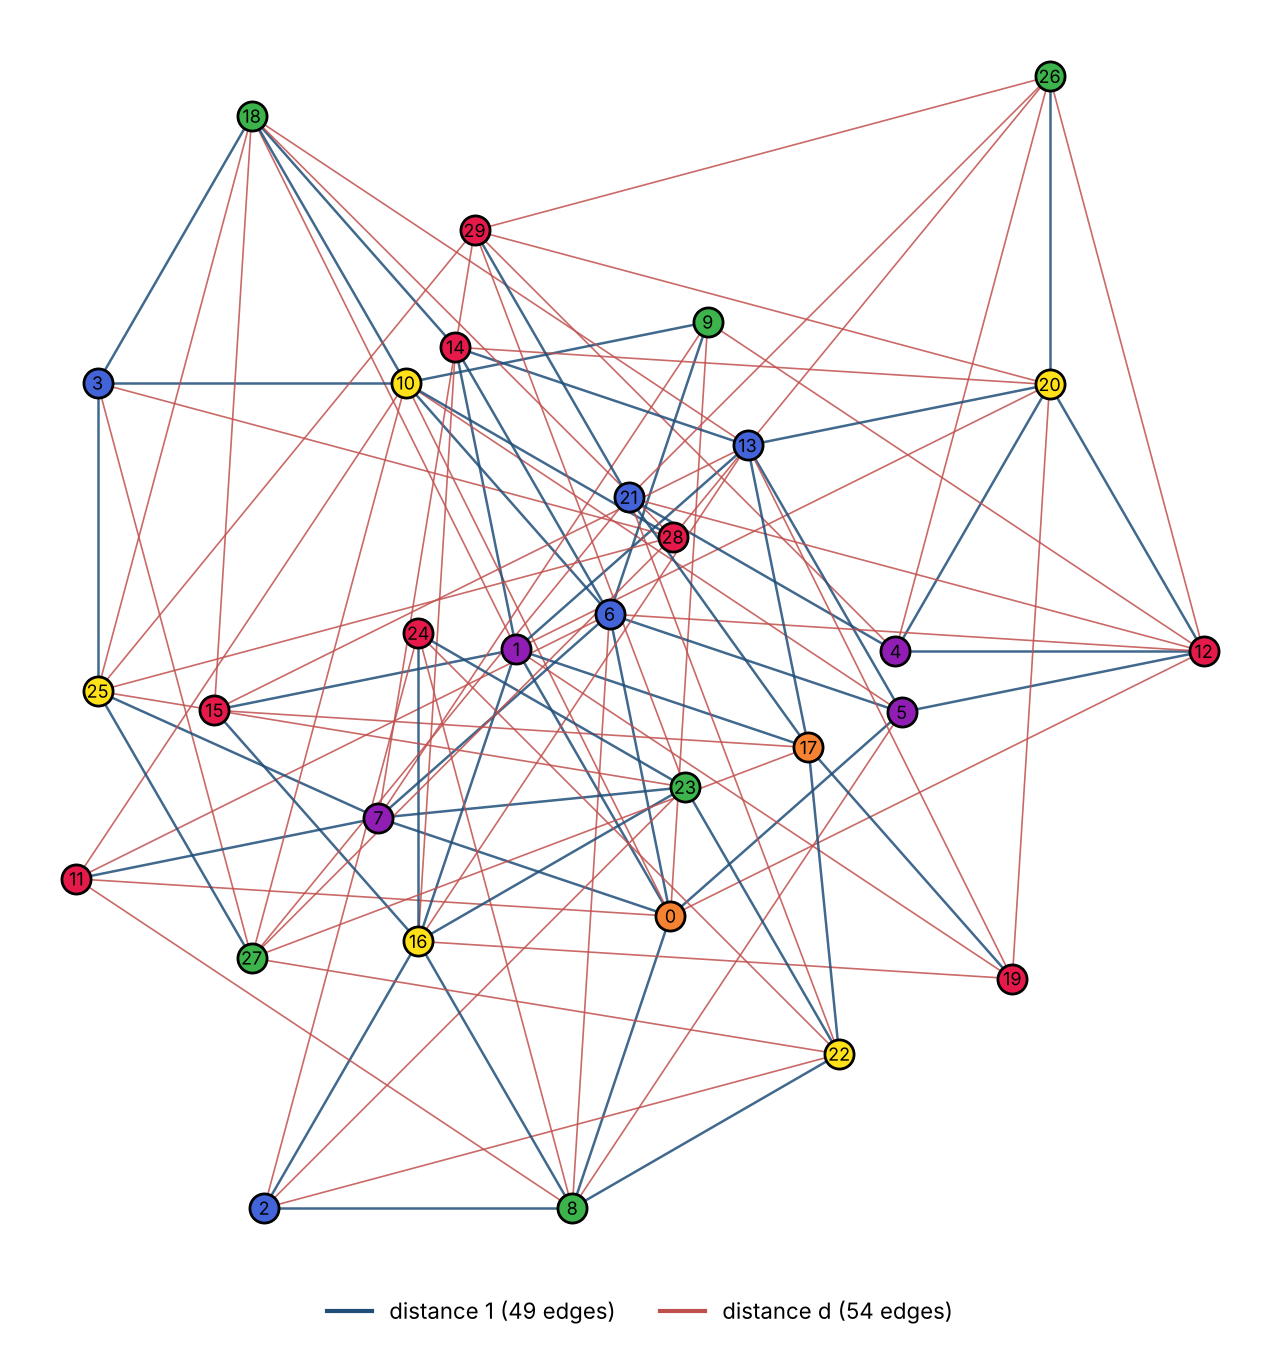
\includegraphics[width=0.66\textwidth]{g30.png}
\caption{$G_{30}$ at its true coordinates. Blue: distance $1$ ($49$ edges); red: distance $d$ ($54$ edges). Vertex colours: the $6$-colouring of Appendix~\ref{app:g30}.}
\label{fig:g30}
\end{figure}

\subsection{Why $\Q(i,\sqrt3)$ is not enough}

\begin{lemma}\label{lem:reduction}
Let $K$ be a CM field with maximal real subfield $K^+$, and $\delta>0$ with $\delta^2\in K^+$. Let $\mathfrak P$ be a prime of $K^+$ inert in $K/K^+$ with residue field $\F_q$, such that $\delta^2$ is a $\mathfrak P$-unit. Then every finite $\{1,\delta\}$-graph with vertices in $K$ maps homomorphically to
\[
H(q,c)=\operatorname{Cay}\bigl(\F_{q^2},\{x:x^{q+1}=1\}\cup\{x:x^{q+1}=c\}\bigr),\qquad c=\delta^2\bmod\mathfrak P.
\]
\end{lemma}

\begin{proof}
Let $\mathfrak p$ be the unique prime of $K$ over $\mathfrak P$; complex conjugation fixes it. An edge vector $v$ has $v\bar v\in\{1,\delta^2\}$, a $\mathfrak P$-unit, and $v,\bar v$ have equal $\mathfrak p$-valuation, so $v$ is a $\mathfrak p$-unit and reduces to a nonzero $x\in\F_{q^2}$. Conjugation induces Frobenius, so $x^{q+1}\in\{1,c\}$. Translating a vertex of each component to $0$ makes all vertices $\mathfrak p$-integral, and reduction is the homomorphism.
\end{proof}

\begin{proposition}\label{prop:zeta12}
Every finite $\{1,d\}$-graph with vertices in $\Q(i,\sqrt3)$ is $4$-colourable; the same holds for $\{1,\sqrt3\}$-graphs.
\end{proposition}

\begin{proof}
The prime $(1+\sqrt3)$ of $\Q(\sqrt3)$ has residue field $\F_2$ and is inert in $\Q(i,\sqrt3)$, and $2+\sqrt3$ and $3$ are units there. In $\F_4$ every nonzero element has norm $1$, so $H(2,c)=K_4$.
\end{proof}

In particular the gadget of Lemma~\ref{lem:gadget}, which lies in $\Q(\zeta)$, is $4$-colourable as a graph ($K_8$ minus a perfect matching), and no finite-graph proof of $\chi(\{1,d\})\ge5$ can live in $\Q(\zeta)$.

\begin{proposition}\label{prop:mod8}
Let $m\ge1$ be squarefree with $3\nmid m$, $K^+=\Q(\sqrt3,\sqrt m)$ and $K=K^+(i)$. The primes of $K^+$ above $2$ have residue field $\F_2$ and are inert in $K/K^+$ if and only if $m\equiv1,2,3,6\pmod 8$. In that case every finite $\{1,d\}$-graph and every finite $\{1,\sqrt3\}$-graph with vertices in $K$ is $4$-colourable.
\end{proposition}

\begin{proof}
All primes above $2$ are conjugate, so it suffices to look at one completion. The square classes of $\Q_2^\times$ are represented by $\pm1,\pm2,\pm5,\pm10$, and $\Q_2(\sqrt a)$ ($a\not\sim1$) is unramified exactly when $a\sim5$. Since $-15\equiv1\pmod8$ is a square in $\Q_2$, $3\sim-5$. Let $V\subset\Q_2^\times/\Q_2^{\times2}$ be generated by $-5$ and $m$; the completion of $K^+$ is $L=\Q_2(\sqrt V)$, and that of $K$ is $L(\sqrt{-1})$. A multiquadratic extension $\Q_2(\sqrt W)$ has residue degree $2$ if $5\in W$ and $1$ otherwise. So the residue field of $L$ is $\F_2$ iff $5\notin V$, and $L(\sqrt{-1})/L$ is inert iff moreover $-1\notin V$ and $5\in\langle V,-1\rangle$. The last condition always holds, since $-5\in V$. Now $V=\{1,-5,m,-5m\}$, and $5\notin V$, $-1\notin V$ together say $m\not\sim5$ and $m\not\sim-1$. For odd $m$ the class of $m$ is that of $m\bmod 8\in\{1,3,5,7\}$, with $3\sim-5$ and $7\sim-1$; even squarefree $m$ is $2$ times an odd unit and is never $\sim5$ or $\sim-1$. This gives exactly $m\equiv1,2,3,6\pmod8$. The colouring statement then follows from Lemma~\ref{lem:reduction} with $q=2$, as in Proposition~\ref{prop:zeta12}, since $2+\sqrt3$ and $3$ are units at $2$.
\end{proof}

This agrees with a direct PARI/GP computation for all $19$ such $m\le38$. The fields of~\cite{DN25} and of this paper ($m=5$ and $m=7$) are exactly of the excluded kind.

\subsection{The upper bound}

\begin{proposition}\label{prop:upper}
$\chi(\{1,d\})\le12$.
\end{proposition}
\begin{proof}
Tile the plane by regular hexagons of diameter $D$ with $d/2<D<1$ (e.g.\ $D=0.98$) and colour them by the cosets of the sublattice spanned by $2(e_1+e_2)$ and $6e_2$ (index $12$), where $e_1,e_2$ generate the lattice of tile centres at angle $60^\circ$. Distinct tiles of the same colour are at distance at least $2D$, so all distances in $[D,2D)\ni1,d$ are avoided.
\end{proof}

This is the standard separation argument and we claim no novelty for it. A computer search over Voronoi tilings of lattices (hexagonal, square and a $9\times10$ grid of other shapes) with sublattices of index $7$ to $11$, testing only the two distances $1$ and $d$, found no colouring with fewer than $12$ colours.

\subsection{Limits of the method}

\begin{proposition}\label{prop:limits}
Let $X$ be a gadget whose pairs at non-forbidden distance form a matching of $m$ pairs, all at distance $\ge\tfrac12$, plus $s$ unmatched points. With $k$ colours it forces $\sum p\ge2m+s-k$ over the matched pairs, and this meets the bound $\sum p\le m/2$ of Lemma~\ref{lem:half} only if $\tfrac32m+s=k$. For $d=(\sqrt2+\sqrt6)/2$ the only solution is $k=6$, $m=4$, $s=0$ ($K_8$ minus a perfect matching). In particular the method of Lemma~\ref{lem:finite} cannot give $\chi(\{1,d\})\ge8$, nor $\chi(\R^2)\ge6$.
\end{proposition}
\begin{proof}
One point from each pair and the unmatched points give $m+s$ points pairwise at distance $1$ or $d$. A planar two-distance set has at most $5$ points, with equality only for the regular pentagon (ratio $(1+\sqrt5)/2\ne d$), so $m+s\le4$. Then $\tfrac32m+s=k$ with $k=6$ forces $m=4,s=0$, and $k=7$ has no solution. For unit distances alone cliques have at most $3$ points, so $m+s\le3$ and $\tfrac32m+s=5$ has no solution.
\end{proof}

A search for such gadgets for $d=\sqrt3$, $2$ and $(1+\sqrt5)/2$ in several rings found none. The general Mixon--Alexeev program of Section~\ref{sec:five}, which contains Lemma~\ref{lem:finite} as a special case, is not subject to this obstruction.



\part{Map-type colourings}

\section{An eleventh trichromatic point}\label{sec:map}

Restricting the shape of colour classes changes the problem. Woodall and Townsend obtained $6$ for map-type colourings and Coulson $6$ for polygonal tilings~\cite{Co04}; Voronov~\cite{Vo24} proved that forbidding an interval $[1-\varepsilon,1+\varepsilon]$ forces $7$ colours, and Sokolov and Voronov~\cite{SV26} adapted the method to map-type colourings and obtained $\chi_{\mathrm{poly}}(\R^2)=7$. We follow~\cite{SV26} for all definitions: a \emph{multicolour} $\bar c(x)$ is the set of colours of regions whose closure contains $x$; $x$ is bichromatic or trichromatic as $|\bar c(x)|=2$ or $3$; $\omega(x)$ is the unit circle about $x$. We use their conditions
\begin{itemize}
\item[C2] boundaries are Jordan curves ending at vertices, and every vertex is an endpoint of at least three boundaries;
\item[C3] every bounded set meets finitely many boundaries;
\item[C5] no boundary contains an arc of a unit circle;
\item[C6] no trichromatic vertex has degree greater than three;
\item[C7] (Section~\ref{sec:radius} only) every vertex has degree exactly three;
\end{itemize}
and, as given, their Lemma~1 (no two bichromatic points with the same multicolour are at distance $1$), Lemma~2 (no point has chromaticity $4$), Lemma~3, Corollary~3 and Proposition~11.

\subsection{The step}
The proof of~\cite[Lemma 4]{SV26} produces ten trichromatic points: a centre $u$ with $\bar c(u)=\{4,5,6\}$ and nine points of multicolours $\{a,b,i\}$, $\{a,b\}\subset\{1,2,3\}$, $i\in\{4,5,6\}$. Two trichromatic points may have neither equal (Lemma~3) nor complementary (Corollary~3) multicolours, so the relevant classes are the $\tfrac12\binom63=10$ complementary pairs of $3$-subsets of $\{1,\dots,6\}$.

\begin{observation}\label{obs:ten}
The ten points are pairwise distinct and pairwise non-complementary, and occupy all ten classes.
\end{observation}

So no contradiction is yet available. The argument of~\cite{SV26} closes with the sentence ``on the boundary of the union of three regions of colours $1,2,3$ whose vertex is $u$, there is at least one more trichromatic point'', without proof; \cite[Lemma 6.1]{Vo24} contains the same step. By Observation~\ref{obs:ten}, the whole contradiction rests on it. (Near $u$ the regions are coloured $4,5,6$; we prove that an eleventh trichromatic point exists, without claiming to reconstruct the intended argument.)

\begin{theorem}\label{thm:eleventh}
Let $c$ be a proper $6$-colouring satisfying C2, C3, C5, C6, and $u$ trichromatic with $\bar c(u)=\{4,5,6\}$. Then there is a trichromatic $v\ne u$ with $\|u-v\|<1$.
\end{theorem}

\begin{proof}
\emph{Step 1.} By C2 and C6, $\deg u=3$; the sectors at $u$ carry $4,5,6$, and exactly one boundary at $u$ separates $4$ from $5$.
\emph{Step 2.} Let $K$ be the component, in the union of all $4|5$ boundaries, containing that boundary. Every $x\in K$ has $\{4,5\}\subseteq\bar c(x)$, and $|\bar c(x)|\le3$ by Lemma~2.
\emph{Step 3.} Suppose $K$ has no trichromatic point other than $u$. Then every vertex $v\ne u$ of $K$ has $\bar c(v)=\{4,5\}$, all its boundaries are $4|5$ boundaries, its sectors alternate, and $\deg_K v=\deg v$ is even and at least $4$; while $\deg_K u=1$.
\emph{Step 4.} If $K$ left the open unit disc about $u$, pick $y\in K\setminus\{u\}$ interior to a boundary and a path in $K$ from $y$ to a point at distance $\ge1$ from $y$; by continuity some point of the path is at distance exactly $1$ from $y$, and both points are bichromatic with multicolour $\{4,5\}$, contradicting Lemma~1. So $K$ lies in the closed unit disc and is a finite graph by C3.
\emph{Step 5.} The degree sum of $K$ is $1+(\text{even})$, odd; contradiction. The trichromatic vertex obtained lies within distance $1$ by Step~4.
\end{proof}

\begin{theorem}\label{thm:odd}
In this situation the number of trichromatic points of $K$ other than $u$ is odd.
\end{theorem}
\begin{proof}
A trichromatic vertex of $K$ has degree $3$ (C6), exactly one of its boundaries is a $4|5$ boundary, so its $K$-degree is $1$; all other vertices have even $K$-degree, and $\deg_K u=1$. A finite graph has an even number of odd vertices.
\end{proof}

\subsection{A case left uncovered}
Here $\bar c(v)=\{4,5,c\}$ with $c\in\{1,2,3,6\}$, never equal to one of the nine points. If $c\in\{1,2,3\}$, $\bar c(v)$ is disjoint from some $p_j$ and Corollary~3 (distance $<2$) applies. If $c=6$, then $u,v$ are trichromatic with the same multicolour at distance $<1$, while~\cite[Lemma 3]{SV26} is stated for distances in $(1,2)$; Corollary~3 does not apply either. This is a gap between what Theorem~\ref{thm:eleventh} delivers and what the cited lemmas consume; it is not a counterexample.

\begin{proposition}\label{prop:degree4}
For any $d$, the unit-distance graph on $\omega(u_1)\cup\omega(u_2)$, $|u_1u_2|=d$, has maximum degree at most $4$.
\end{proposition}
\begin{proof}
For $x\in\omega(u_1)$, the unit circle $\omega(x)$ meets $\omega(u_1)$ in the two points at $\pm60^\circ$ and $\omega(u_2)$ in at most two points.
\end{proof}
So the natural route of extending Lemma~3 below $1$ through $3$-colourability of $\omega(u_1)\cup\omega(u_2)$ is closed.

\section{The obstruction radius}\label{sec:radius}

Let $\rho$ be the least radius such that every closed disc of radius $\rho$ contains a trichromatic point; \cite[\S7]{SV26} assert $\rho\le1$ without argument and ask (Question~1) for the least area of a convex region in which their conclusion can be asserted.

\begin{theorem}\label{thm:radius}
The argument of~\cite{SV26} requires exactly the disc $D(x,\rho+2)$ about any point $x$: a trichromatic $u$ within $\rho$ of $x$, the unit circle $\omega(u)$ with an annulus of width $\eta\to0$, and a second trichromatic point $u_2$ inside $\omega(u)$ with its annulus. With $\rho=1$ this is the radius $3$ of~\cite{SV26}.
\end{theorem}

\begin{theorem}\label{thm:disc}
The convex region of least area in which the conclusion can be asserted by this argument is a disc, of area $\pi(\rho+2)^2$.
\end{theorem}
\begin{proof}
The requirement is $D(x,\rho+2)\subseteq K$; area is monotone under inclusion.
\end{proof}

For comparison, the least areas of other shapes containing a disc of radius $3$: regular hexagon $31.18$ ($1.10\times$), Reuleaux triangle $35.51$ ($1.26\times$; its inradius is only $w(1-1/\sqrt3)$), square $36$, equilateral triangle $46.77$.

\begin{theorem}\label{thm:rho1}
Under C7, $\rho<1$.
\end{theorem}
\begin{proof}
In a disc $D$ of radius $\rho$ with no trichromatic point there is no degree-$3$ vertex (its three sectors are pairwise adjacent, hence pairwise distinct in colour), hence under C7 no vertex. So $D$ is cut by disjoint Jordan arcs with endpoints on $\partial D$; each face meets $\partial D$, is monochromatic and connected, so has diameter $<1$; the face of the centre then has diameter $\ge\rho$.
\end{proof}

\begin{lemma}\label{lem:twocol}
Let $D$ be a trichromatic-free disc in which every face meets a vertex and the diagonal-adjacency graph (faces at a common vertex in the same checkerboard class) is connected. Then $D$ carries exactly two colours.
\end{lemma}
\begin{proof}
All vertices have even degree, so the faces have a proper $2$-colouring $\chi$; at each vertex the true colours alternate along $\chi$-classes, and connectivity propagates this.
\end{proof}

\begin{corollary}\label{cor:half}
Under the hypothesis of Lemma~\ref{lem:twocol}, $D$ has radius at most $\tfrac12$.
\end{corollary}
\begin{proof}
The star polygons $\{(2k+1)/k\}$ with unit edges are odd unit-distance cycles with circumradius $R_k=1/(2\sin(k\pi/(2k+1)))\to\tfrac12$.
\end{proof}

\begin{theorem}\label{thm:chords}
Let $D$ be a disc of radius $\rho\ge1/\sqrt3$ cut by pairwise disjoint Jordan arcs with endpoints on $\partial D$. Then some face has diameter at least $\rho\sqrt3$.
\end{theorem}
\begin{proof}
Take $P_1,P_2,P_3\in\partial D$ at mutual angle $2\pi/3$, pairwise at distance $\rho\sqrt3\ge1$, and suppose every face has diameter $<1$; then they lie in distinct faces $F_1,F_2,F_3$. The faces form a tree under adjacency; let $F_m$ be the median of $F_1,F_2,F_3$. For each $P_i\notin F_m$ a bounding arc of $F_m$ cuts off a rim arc $B_i\ni P_i$; the $B_i$ are disjoint, so the rim contact of $F_m$ interleaves $P_1,P_2,P_3$ and contains two points at angular distance $\ge2\pi/3$, hence at distance $\ge\rho\sqrt3\ge1$. The case $F_m=F_i$ is the same.
\end{proof}

\begin{corollary}\label{cor:rho}
$\rho\le1/\sqrt3\approx0.5774$. Hence the radius required by~\cite{SV26} is $2+1/\sqrt3\approx2.5774$, and the answer to their Question~1 is $\pi(2+1/\sqrt3)^2\approx20.87$, against $9\pi\approx28.27$.
\end{corollary}
\begin{proof}
A trichromatic-free disc is vertex-free, and Theorem~\ref{thm:chords} caps its radius at $1/\sqrt3$, or vertex-bearing, and Corollary~\ref{cor:half} caps it at $\tfrac12$.
\end{proof}

The remaining uncertainty is $\tfrac12\le\rho\le1/\sqrt3$, and it concerns vertex-free arrangements only. A search over arrangements of disjoint chords never produced a face whose rim contact spanned less than about $136^\circ$, suggesting $\rho\lesssim0.539$; we have no proof. The combinatorial content of this part was checked by self-contained scripts ($99$ assertions), and Propositions~6, 12, Lemma~2 and Corollary~4 of~\cite{SV26} were reproduced independently.

\part{The unit sphere}

\section{\texorpdfstring{$\alpha(3,\tfrac12)=7$}{alpha(3,1/2)=7}}\label{sec:sphere}

Let $S^2(r)$ carry the graph joining points at Euclidean distance $1$. Let $h$ be the largest number of points of $S^2(1)$ whose chord-$1$ graph has independence number at most $2$ (an almost-equidistant set of unit chords). A unit chord means inner product $\tfrac12$, so in the notation of Bachoc, Bekker, Moustrou and de Oliveira Filho~\cite{BBMO25} $h=\alpha(3,\tfrac12)$. Their results concern $t\le0$, and they note that their bound $\alpha(n,t)\le2(n+1)$ fails for some positive $t$. Rosenfeld~\cite{Ro91} and Bezdek--L\'angi~\cite{BL99} treat radii below $1/\sqrt2$.

\begin{lemma}\label{lem:K4free}
The chord-$1$ graph on $S^2(1)$ contains no $K_4$.
\end{lemma}
\begin{proof}
Four mutually adjacent unit vectors would have Gram matrix $\tfrac12(I+J)$, positive definite, hence would be linearly independent in $\R^3$.
\end{proof}

\begin{theorem}\label{thm:h8}
$h\le8$.
\end{theorem}
\begin{proof}
The graph has no $K_4$ (Lemma~\ref{lem:K4free}) and its complement is triangle-free; $R(3,4)=9$.
\end{proof}

The $(3,4)$-Ramsey graph on $8$ vertices is unique: the complement of the Wagner graph. For realisability we use a triangle $\{a,b,c\}$ as a basis (Gram matrix $M=\tfrac12(I+J)$, invertible): with $t_v=(\langle v,a\rangle,\langle v,b\rangle,\langle v,c\rangle)^T$, $\langle u,v\rangle=t_u^TM^{-1}t_v$, and realisability becomes a polynomial system with one equation $|v|^2=1$ per remaining vertex and one equation $\langle u,v\rangle=\tfrac12$ per remaining edge, non-edges left free.

\begin{theorem}\label{thm:n8}
The complement of the Wagner graph is not realisable on $S^2(1)$. Hence $h\le7$.
\end{theorem}
\begin{proof}
With the triangle $\{0,2,5\}$ the system has $12$ equations in $9$ unknowns over $\Q$, and its Gr\"obner basis (grevlex) is $\{1\}$: no solution even over $\C$.
\end{proof}

\begin{theorem}[{\cite[Thm.~5.2(11)]{BBMO25}}]\label{thm:h7lower}
$h\ge7$: the spindle $MS(2)$, of order $7$, is $(3,t)$-realisable for $t\ge t_{2,3}=0.255338\ldots$, the largest root of $32t^3+15t^2-2t-1$.
\end{theorem}

\begin{corollary}
$\alpha(3,\tfrac12)=7$.
\end{corollary}

\begin{theorem}[uniqueness]\label{thm:unique7}
Among the $13{,}842$ labelled graphs on $7$ vertices with $\alpha\le2$ and $\omega\le3$ there are $9$ isomorphism classes, and exactly one, $MS(2)$ ($11$ edges, degree sequence $[3,3,3,3,3,3,4]$), is realisable on $S^2(1)$; the other eight give Gr\"obner basis $\{1\}$.
\end{theorem}

\begin{theorem}[explicit realisation]\label{thm:Q46}
$MS(2)$ is realised over $\Q(\sqrt{46})$ by the Gram matrix with $1$ on the diagonal, $\tfrac12$ on the $11$ edges, and on the ten non-edges the values $-\tfrac13$, $\tfrac{37}{64}$, $\tfrac18\pm\tfrac{\sqrt{46}}{16}$, $\tfrac{23}{64}\pm\tfrac{3\sqrt{46}}{32}$. It has rank $3$ and eigenvalues $\tfrac{57}{32}$, $\tfrac{167}{64}\pm\tfrac{\sqrt{21881}}{192}$ and $0$ (multiplicity $4$), so it is the Gram matrix of seven unit vectors in $\R^3$; no non-edge entry equals $\tfrac12$. By~\cite[Lemma 5.1]{BBMO25} the realisation is unique up to isometry.
\end{theorem}

\subsection{Two structural facts}
Let $\alpha$ be the angle subtended by a unit chord on $S^2(r)$. Two neighbours of a vertex at azimuthal separation $\Delta$ are adjacent iff $\cos\Delta=\cos\alpha/(1+\cos\alpha)$, and the link is a cycle $C_k$ iff $\Delta=2\pi/k$. This happens exactly for $k=3,4,5$, at the circumradii $0.612372$, $0.707107$, $0.951057$ of the tetrahedron, octahedron and icosahedron ($k=6$ is the plane in the limit, where the link is de Grey's hexagon).

\begin{theorem}\label{thm:nocycle}
On $S^2(1)$ the link of every vertex is a disjoint union of paths.
\end{theorem}
\begin{proof}
At $r=1$, $\alpha=60^\circ$ and $\cos\Delta=\tfrac13$. By Niven's theorem $\Delta/\pi$ is irrational, so $k\Delta\ne2\pi m$.
\end{proof}

This closes the cone route to $\chi(\R^3)\ge7$ via $\chi(\R^3)\ge1+\chi(S^2(1))$: the cone needs radius $1$, while the only wheel gadget lives at the icosahedral radius. In higher dimensions the same argument gives $h_d\le R(3,d+1)-1$ ($13,17,22$ for $d=4,5,6$), against $2d+1$ from the spindles $MS(d-1)$.

\section{Open problems}\label{sec:open}

\begin{enumerate}
\item \emph{Two distances.} Close $7\le\chi(\{1,(\sqrt2+\sqrt6)/2\})\le12$. By Proposition~\ref{prop:limits} the ``exactly $\tfrac12$'' method cannot give $8$; the general Mixon--Alexeev program might, at a scale needing column generation with a MaxSAT pricing step.
\item \emph{Other distances.} Prove $\chi(\{1,\sqrt3\})\ge7$; no $8$-point gadget of the required type exists in the rings we searched.
\item \emph{Smaller certificates.} Is there a certificate for Theorem~\ref{thm:seven} much smaller than $262$ points, or a $6$-chromatic $\{1,d\}$-graph with fewer than $30$ vertices?
\item \emph{The semi-mono programme} (P\'alv\"olgyi and de Grey, thread~12): minimise the $409$-vertex graph under the relaxation that allows a few non-unit edges where $0<p_\delta<\tfrac12$.
\item \emph{Forcing $p_{1/\sqrt3}$ exactly} (de Grey, thread~5), and its $k=5$ analogue via Lemma~\ref{lem:hexagon}.
\item \emph{Concentrated unit hexagons}: a closed unit hexagon whose nine diagonals take two or three values.
\item \emph{An analogue of Polymath16 Proposition~36} (bounds on whole intervals of distances) at $k=5$.
\item \emph{Map-type colourings}: determine $\rho\in[\tfrac12,1/\sqrt3]$; decide whether two trichromatic points can share a multicolour at distance $<1$.
\item \emph{The sphere}: is $\chi(S^2(1))=4$? Is $h_d\le R(3,d+1)-1$ far from tight for $d\ge4$? A direct proof of uniqueness at $n=7$.
\end{enumerate}

\section*{Data availability}
Ancillary files: \texttt{cert7.json} and \texttt{rup\_checker.c} (Theorem~\ref{thm:seven}); \texttt{g30\_two\_distance.json} (Theorem~\ref{thm:g30}); \texttt{verify\_hull.py}, \texttt{build\_g17.py}, \texttt{certificate.json}, \texttt{check\_certificate.py}, \texttt{certificate19.json}, \texttt{check\_certificate19.py} (Section~\ref{sec:five}); \texttt{h\_sphere.py}, \texttt{h7.py}, \texttt{h7\_gram.py}, \texttt{h7\_theorem.py}, \texttt{h8\_impossible.py} (Section~\ref{sec:sphere}). The CNF and DRUP proof for Theorem~\ref{thm:seven} ($\approx97$\,MB) are available from the author; the proof was checked by two independent checkers (\texttt{drat-trim} and \texttt{rup\_checker.c}).

\section*{Acknowledgements}
Much of the search, minimisation and verification code was developed with the assistance of Claude (Anthropic). All claims were checked as described; the author takes responsibility for the content.

\bibliographystyle{amsplain}
\bibliography{refs}

\appendix
\section{The graph $G_{30}$}\label{app:g30}

Vertex $v$ is $z=(a_0+a_1\sqrt3+a_2\sqrt7+a_3\sqrt{21})/8+i\,(b_0+b_1\sqrt3+b_2\sqrt7+b_3\sqrt{21})/8$. The last column is a proper $6$-colouring.

{\small
\begin{longtable}{rllll}
\toprule
$v$ & $(a_0,a_1,a_2,a_3)$ & $(b_0,b_1,b_2,b_3)$ & neighbours & colour\\
\midrule
\endhead
0 & $(8, 0, 0, 0)$ & $(0, 0, 0, 0)$ & 1, 5, 6, 7, 8, 9, 10, 11, 12 & 5 \\
1 & $(4, 0, 0, 0)$ & $(0, 4, 0, 0)$ & 0, 13, 14, 15, 16, 17, 18, 19, 20 & 6 \\
2 & $(0, -3, 1, 0)$ & $(-3, 0, 0, -1)$ & 8, 16, 22, 23, 24 & 4 \\
3 & $(3, 0, -2, -1)$ & $(6, 3, 1, 0)$ & 10, 18, 25, 27, 28 & 4 \\
4 & $(6, 3, 1, 0)$ & $(-3, 0, 2, 1)$ & 12, 20, 21, 26, 29 & 6 \\
5 & $(14, 0, 0, 0)$ & $(0, 0, 2, 0)$ & 0, 6, 8, 10, 12, 13 & 6 \\
6 & $(11, 0, 0, -1)$ & $(0, 3, 1, 0)$ & 0, 5, 7, 8, 9, 10, 11, 12, 14 & 4 \\
7 & $(5, 0, 0, -1)$ & $(0, 3, -1, 0)$ & 0, 6, 9, 11, 23, 25, 29 & 6 \\
8 & $(8, -3, 1, 0)$ & $(-3, 0, 0, -1)$ & 0, 2, 5, 6, 11, 16, 22, 24 & 2 \\
9 & $(11, 3, -1, -1)$ & $(3, 3, 1, 1)$ & 0, 6, 7, 10, 12 & 2 \\
10 & $(11, 0, -2, -1)$ & $(6, 3, 1, 0)$ & 0, 3, 5, 6, 9, 11, 18, 27, 28 & 3 \\
11 & $(5, -3, -1, -1)$ & $(3, 3, -1, -1)$ & 0, 6, 7, 8, 10 & 1 \\
12 & $(14, 3, 1, 0)$ & $(-3, 0, 2, 1)$ & 0, 4, 5, 6, 9, 20, 21, 26 & 1 \\
13 & $(10, 0, 0, 0)$ & $(0, 4, 2, 0)$ & 1, 5, 14, 15, 16, 17, 18, 19, 20 & 4 \\
14 & $(7, 0, 0, -1)$ & $(0, 7, 1, 0)$ & 1, 6, 13, 16, 18, 20 & 1 \\
15 & $(4, -3, -1, 0)$ & $(3, 4, 0, -1)$ & 1, 13, 16, 17, 18 & 1 \\
16 & $(4, -3, 1, 0)$ & $(-3, 4, 0, -1)$ & 1, 2, 8, 13, 14, 15, 19, 23, 24 & 3 \\
17 & $(7, 0, 0, 1)$ & $(0, 1, 1, 0)$ & 1, 13, 15, 19, 21, 22, 27 & 5 \\
18 & $(7, 0, -2, -1)$ & $(6, 7, 1, 0)$ & 1, 3, 10, 13, 14, 15, 25, 28 & 2 \\
19 & $(7, 0, 2, 1)$ & $(-6, 1, 1, 0)$ & 1, 13, 16, 17, 20 & 1 \\
20 & $(10, 3, 1, 0)$ & $(-3, 4, 2, 1)$ & 1, 4, 12, 13, 14, 19, 26, 29 & 3 \\
21 & $(6, -1, 1, 0)$ & $(1, 0, 2, 1)$ & 4, 12, 17, 22, 26, 27, 29 & 4 \\
22 & $(8, 1, 1, 0)$ & $(1, 0, 0, -1)$ & 2, 8, 17, 21, 23, 24, 27 & 3 \\
23 & $(4, 1, 1, 0)$ & $(1, 4, 0, -1)$ & 2, 7, 16, 22, 24, 25, 29 & 2 \\
24 & $(4, -3, 1, 0)$ & $(5, 4, 0, -1)$ & 2, 8, 16, 22, 23 & 1 \\
25 & $(3, 0, -2, -1)$ & $(-2, 3, 1, 0)$ & 3, 7, 18, 23, 27, 28, 29 & 3 \\
26 & $(10, 3, 1, 0)$ & $(5, 4, 2, 1)$ & 4, 12, 20, 21, 28, 29 & 2 \\
27 & $(7, 0, -2, -1)$ & $(-2, -1, 1, 0)$ & 3, 10, 17, 21, 22, 25, 28 & 2 \\
28 & $(11, 4, -2, -1)$ & $(2, 3, 1, 0)$ & 3, 10, 18, 25, 26, 27 & 1 \\
29 & $(2, -1, 1, 0)$ & $(1, 4, 2, 1)$ & 4, 7, 20, 21, 23, 25, 26 & 1 \\
\bottomrule
\end{longtable}
}



\end{document}
